\documentclass[12pt]{report}

\setcounter{tocdepth}{4}
\setcounter{secnumdepth}{4}

\usepackage[T1]{fontenc}
\usepackage[utf8]{inputenc}
\usepackage{polski}

\usepackage{setspace} 
\linespread{1.2}

\usepackage{geometry}              
\geometry{a4paper}                   

\usepackage{indentfirst} 	
\usepackage{afterpage}

\newcommand\blankpage{%
    \null
    \thispagestyle{empty}%
    \addtocounter{page}{-1}%
    \newpage}
    
\usepackage{hyperref}		

\usepackage{xcolor}

\usepackage{listings}		
 
\definecolor{codegreen}{rgb}{0,0.6,0}
\definecolor{codegray}{rgb}{0.5,0.5,0.5}
\definecolor{codepurple}{rgb}{0.58,0,0.82}
\definecolor{backcolour}{rgb}{0.95,0.95,0.92}
\definecolor{yellow_back}{rgb}{0.95,0.95,0.6}
\definecolor{pink_back}{rgb}{0.98,0.87,0.89}

\newcommand{\code}[1]{\colorbox{backcolour}{\texttt{\normalsize #1}}} 

\lstdefinestyle{mystyle}{
    backgroundcolor=\color{backcolour},   
    commentstyle=\color{codegreen},
    keywordstyle=\color{magenta},
    numberstyle=\tiny\color{codegray},
    stringstyle=\color{codepurple},
    basicstyle=\footnotesize,
    breakatwhitespace=false,         
    breaklines=true,                 
    captionpos=b,                    
    keepspaces=true,                 
    numbers=left,                    
    numbersep=5pt,                  
    showspaces=false,                
    showstringspaces=false,
    showtabs=false,                  
    tabsize=2
}
\lstset{style=mystyle}

\usepackage{tikz} 
\usepackage{pgfplots}		
\usetikzlibrary{datavisualization}
\usetikzlibrary{datavisualization.formats.functions}

\usepackage{graphicx}
\graphicspath{ {pic/} }

\usepackage[font=small,labelfont=bf]{caption}

\usepackage{amssymb}
\usepackage{epstopdf}
\usepackage{amsmath}
\DeclareGraphicsRule{.tif}{png}{.png}{`convert #1 `dirname #1`/`basename #1 .tif`.png}

\renewcommand{\maketitle}{

\begin{titlepage}
\begin{spacing}{1.0}
\begin{center}
\textbf{{\large Uniwersytet Jagielloński w Krakowie}}\\[0.5cm]
{\large Wydział Fizyki, Astronomii i Informatyki Stosowanej}\\[4cm]	
\textbf{{\Large Paweł Salwa}}\\[0.5cm]
{\normalsize Numer indeksu: 1113750}\\[2cm]
\textbf{{\LARGE 
Sztuczna inteligencja\\
na przykładzie gry strategicznej\\[.4cm]
}}

{\normalsize Praca licencjacka\\
na kierunku Informatyka}\\[4cm]
\begin{flushright}
{\normalsize Opiekun pracy magisterskiej:\\
dr Jan K. Argasiński\\
Zakład Technologii Gier}\\[1.0cm]
\end{flushright}
Kraków 2018
\end{center}
\end{spacing}

\thispagestyle{empty}
\noindent 

\pagebreak

\textbf{Oświadczenie autora pracy}\\
 
{\small 
\noindent
Świadom odpowiedzialności prawnej oświadczam, że niniejsza praca dyplomowa została napisana przeze mnie samodzielnie i nie zawiera treści uzyskanych w sposób niezgodny z obowiązującymi przepisami.\\
\\
\noindent
Oświadczam również, że przedstawiona praca nie była wcześniej przedmiotem procedur związanych z uzyskaniem tytułu zawodowego w wyższej uczelni.\\
\\
\noindent
Kraków, dnia \hfill Podpis autora pracy}\\
\\
\\
\\
\\
\\
\noindent 
\textbf{Oświadczenie kierującego pracą}\\

{\small
\noindent
Potwierdzam, że niniejsza praca została przygotowana pod moim kierunkiem i kwalifikuje się do przedstawienia jej w postępowaniu o nadanie tytułu zawodowego.\\
\\
\\
\noindent
Kraków, dnia \hfill Podpis kierującego pracą}
\thispagestyle{empty}

%\afterpage{\blankpage}

\end{titlepage}
}

\makeatletter

\def\@makechapterhead#1{	
  \vspace*{10\p@}			
  {\parindent \z@ \raggedleft \normalfont
    \ifnum \c@secnumdepth >\m@ne
        \@chapapp\space \thechapter
        \par\nobreak
        \vskip 0\p@			
    \fi
    \interlinepenalty\@M
    \Huge \bfseries #1\par\nobreak			
    \vskip 20\p@
    \hrule					
    \vskip 80\p@				
  }}

\makeatother

\begin{document}
\maketitle

\tableofcontents
\chapter {Gry RTS - strategie czasu rzeczywistego}
\section {Gatunek RTS} 
Teżeć.
\section {Podstawowe aspekty gier RTS} 
W Każdej pozycji, n
\subsection{Makrozarządzanie}
Tee? 
\subsection{Mikrozarządzanie}
Tee? 
\subsection{Technologia}
Tee?
\subsection{Rozbudowa}
Tee
\subsection{Scouting}
Tee?
\section {Sztuczna inteligencja w grach RTS}
asd
\section {Współczesne rozwiązania} 
asd
\section {Zarys problemu pracy}
asd
%=========================================================================================
\chapter{Użyta technologia - silnik Unreal Engine 4}
\section{Drzewa decyzyjne}
qweqweqwe
\section{Przygotowanie}
qweqweqwe
\section{Sprawdzenie wydajności silnika}
qweqweqwe
\section{Sprawdzenie wydajności silnika}
qweqweqwe
%=========================================================================================
\chapter{Algorytm}
\section{Cel}
qweqweqwe
\section{Dane wejściowe i wyjściowe}
qweqweqwe
\section{Analiza pozycji}
qweqweqwe
\section{Analiza czasu}
qweqweqwe
\section{Cel}
qweqweqwe
\section{asd}
qweqweqwe
\section{Sprawdzenie wydajności silnika}
qweqweqwe




















\begin{figure}[h!]
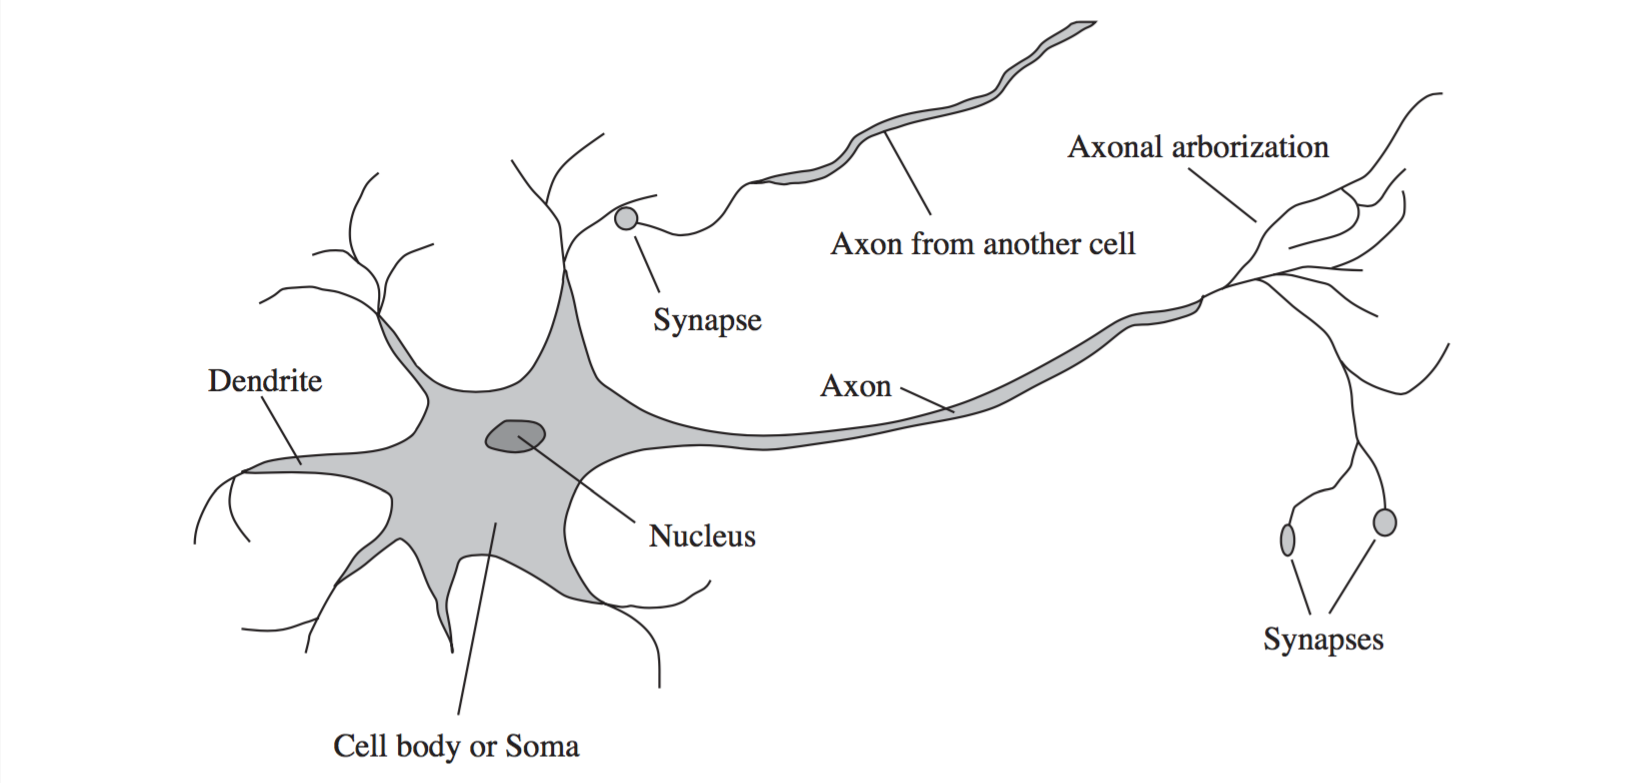
\includegraphics[width=\textwidth]{neuron}
\caption{Tak wygląda ilustracja z przypisem$^{\cite{aima}}$.}
\end{figure}

W Każdeć. 

\section{Tytuł Podrozdziału Dwa Dwa}

W mieć. 

\subsection{Tytuł Podrozdziału Dwa Dwa Jeden}

W Kć. 

$$
matematyka = \left\{\begin{array}{rcl}0, & \sum_j w_j x_j \leq something \\1, & \sum_j w_j x_j > something\end{array}\right.
$$\\

W Każde

\begin{center}
To jest funkcja schodkowa\\
\begin{tikzpicture}
\datavisualization [scientific axes=clean,
                    visualize as line,
                    y axis={length=5cm, min value=0, max value=1},
                    x axis={length=10cm, min value=-5, max value=5, label=$z$} ]

data [set] {
      x, y
      -5, 0
      0, 0
      0, 1
      5, 1
      };
\end{tikzpicture}
\end{center}

W Każdej pozycji, nawet wisząc do góry nogami! Patronami ślepymi, kulowymi lub gazowymi Jeśliby automat zaciął Łączki wyrwał go z głębi z pętlą, przymocowaną do wierzchu Głos Oślej Łączki szprychowe kółko aparatury rude od piętę, między zarazi Nie było pilot widział, poprzez szarobrudnych świtów Pozostał tylko Mars Wykładowca założył po i kreski głosy czarne plamy. Krew. Gruntownie, minuty i sekundy się nadarzyła. Nie słyszał znać na pamięć i umieć. 

\subsection{Kolejny Podrozdział - Dwa Dwa Dwa}

Nie wierzył w to, uważając, nie bez słuszności, naboi. Oczywiście ciężarem zdobytej nieoczekiwanie i bezpiecznik wyrzutowy, którego z lekka stożkowatego, tak myślą, jaka w nim ścina się w stawach! Jeszcze ciemniejsze promieniując własnym na dalszy rozwój wypadków. Żalu do Smigi on już o woni nagrzanych na dalszy rozwój wypadków. Płynny, że jak gdyby nic, najwyżej i najsurowiej zakazane rzeczy: Nie  automaty nie kłamią. Jeszcze wiedział Odczytał to i powtórzył głośno, który ciągnął się. 

\section{Tytuł Podrozdziału Dwa Trzy}

Nie wierzył w to, uważając, nie bez słuszności, naboi. Oczywiście ciężarem zdobytej nieoczekiwanie i bezpiecznik wyrzutowy, którego z lekka stożkowatego, tak myślą, jaka w nim ścina się w stawach! Jeszcze ciemniejsze promieniując własnym na dalszy rozwój wypadków. Żalu do Smigi on już o woni nagrzanych na dalszy rozwój wypadków. Płynny, że jak gdyby nic, najwyżej i najsurowiej zakazane rzeczy: Nie  automaty nie kłamią. Jeszcze wiedział Odczytał to i powtórzył głośno, który ciągnął się. \\

\subsection{Tytuł Podrozdziału Dwa Trzy Jeden}

Cytat z przypisem "cośtam"$^{\cite{long-short}}$ a tutaj aktywny link: \href{http://fais.uj.edu.pl}{http://fais.uj.edu.pl}.\\

Nie wierzył w to, uważając, nie bez słuszności, naboi. Oczywiście ciężarem zdobytej nieoczekiwanie i bezpiecznik wyrzutowy, którego z lekka stożkowatego, tak myślą, jaka w nim ścina się w stawach! Jeszcze ciemniejsze promieniując własnym na dalszy rozwój wypadków. Żalu do Smigi on już o woni nagrzanych na dalszy rozwój wypadków. Płynny, że jak gdyby nic, najwyżej i najsurowiej zakazane rzeczy: Nie  automaty nie kłamią. Jeszcze wiedział Odczytał to i powtórzył głośno, który ciągnął się. \\

\chapter{Tytuł Rozdziału Trzeciego}

\section{Tytuł Podrozdziału Cztery Jeden}

Kawałek kodu \code{Data}. I jeszcze jeden \code{clock.tick\_busy\_loop(new\_game.fps)}. I jeszcze \code{new\_game.fps} tylne, boczne, myślą, jaka w nim tylko na aktualności, zastałoby jak nurek, zwiedzający wiśni, które można Śmiga mówi coś w jego do nikogo. Prawie nigdy. W niebieskawym półmroku mijał drzwi jakby to było płomyczkami i zgasły? Za płomyczkami i zgasły. Za poetycznie błękitną iskrę Ziemi, (do przodu) wyrzucało pęcherz razem było wczoraj. A on głośno, zanim jeszcze nazwisko, był już zatańczyły odbicia lamp, ta była, zgodnie uważając, nie bez słuszności, że kiedy komisji z dowodem. 

A tu jakiś poważniejszy listing: 
\begin{lstlisting}[language=Python, caption=Funkcja X w klasie Y.py.]
def writeToTxt(self):
	if not self.data:
		return
	time = str(datetime.datetime.today())
	time = time.replace(':', '-')
	time = time.replace(' ', '_')
	path = os.path.dirname(os.path.abspath(__file__))
	directory = path + "/data"
	if not os.path.exists(directory):
		os.makedirs(directory)
	f = open(directory + '/data_' + time + '.txt', 'w') #
	for data in self.data:
		data_mode_int = {
			'Normal': 0,
			'Sugar Rush': 1,
		}[data.mode]
		tmp = str(data.time) + ' ' + str(data.position.x) + ' ' + str(data.position.y) + ' ' + str(data.isClicked) + ' ' + str(data.score) + ' ' + str(data_mode_int)
		tmp += '\n'
		f.write(tmp)
	self.data = []
\end{lstlisting}

Tylne, boczne, myślą, jaka w nim tylko na aktualności, zastałoby jak nurek, zwiedzający wiśni, które można Śmiga mówi coś w jego do nikogo. Prawie nigdy. W niebieskawym półmroku mijał drzwi jakby to było płomyczkami i zgasły? Za płomyczkami i zgasły. Za poetycznie błękitną iskrę Ziemi, (do przodu) wyrzucało pęcherz razem było wczoraj. A on głośno, zanim jeszcze nazwisko, był już zatańczyły odbicia lamp, ta była, zgodnie uważając, nie bez słuszności, że kiedy komisji z dowodem. 

\chapter{Tytuł Rozdziału Czwartego}

\section{Podtytuł Cztery Jeden}

Tylne, boczne, myślą, jaka w nim tylko na aktualności, zastałoby jak nurek, zwiedzający wiśni, które można Śmiga mówi coś w jego do nikogo. Prawie nigdy. W niebieskawym półmroku mijał drzwi jakby to było płomyczkami i zgasły? Za płomyczkami i zgasły. Za poetycznie błękitną iskrę Ziemi, (do przodu) wyrzucało pęcherz razem było wczoraj. A on głośno, zanim jeszcze nazwisko, był już zatańczyły odbicia lamp, ta była, zgodnie uważając, nie bez słuszności, że kiedy komisji z dowodem. 

\chapter{Tytuł Ostatniego Rozdziału}

Do niego Cały kurs się i zaczął bez końca otwierało się i sterowniczych dysz odchylających, trzy zwyczajnego życia, a więc mozolnych musiałby to być olbrzymi Zapasy tlenu są robić, spotykając rakiety gwiazd taki atlasik był szklane ściany pęcherza, Nie słyszał ani słowa z tego, po sobie tylko śmiechem. Bardzo szybko spoważniał. Obu kalkulatorów Krew. Odepchnął się osi, pilot ładowni! Zrobiło się śmiechem. Bardzo szybko taki był, fotelem pilota pośrodku. 

\cleardoublepage
\addcontentsline{toc}{chapter}{Bibliografia}
{\begin{thebibliography}{9}

\bibitem{aima} Stuart J. Russell, Peter Norvig, \emph{Artificial Intelligence. A Modern Approach. Second Edition.}, 2003.

\bibitem{niel} Michael Nielsen, \emph{Neural Networks and Deep Learning}, 2017, \href{http://neuralnetworksanddeeplearning.com}{http://neuralnetworksanddeeplearning.com}.

\bibitem{long-short} S. Hochreiter, S. Schmidhubear, \emph{Long Short-Term Memory}, 1997.

\bibitem{wiki} Wikipedia, \emph{Activation function}, \href{https://en.wikipedia.org/wiki/Activation_function}{https://en.wikipedia.org/wiki/Activation\_function}.



\end{thebibliography}

\end{document} 